\documentclass[10pt,twocolumn]{article}

\usepackage[a4paper,margin=1.9cm]{geometry}
\usepackage{times}
\usepackage{graphicx}
\usepackage{booktabs}
\usepackage{caption}
\usepackage{amsmath}
\usepackage{hyperref}
\usepackage{titlesec}
\usepackage{abstract}
\usepackage{enumitem}
\usepackage{xcolor}

\hypersetup{colorlinks=true, linkcolor=blue, urlcolor=blue, citecolor=blue}

\titleformat{\section}{\large\bfseries}{\thesection}{1em}{}
\titleformat{\subsection}{\normalsize\bfseries}{\thesubsection}{1em}{}
\titlespacing{\section}{0pt}{8pt}{4pt}
\titlespacing{\subsection}{0pt}{6pt}{3pt}

\setlength{\abovecaptionskip}{4pt}
\setlength{\belowcaptionskip}{2pt}
\captionsetup{font=small,labelfont=bf}

\renewcommand{\abstractnamefont}{\normalfont\bfseries}
\renewcommand{\abstracttextfont}{\normalfont\itshape}

\title{\textbf{Data-Driven Analysis of the Indian Mutual Fund Industry:\\
A Risk--Return and Investor Behaviour Study}}

\author{
Hariharan S \\
\small Department of Computer Science and Engineering \\
\small IIITDM Kurnool, Kallakurichi, Tamil Nadu, India \\
\small \texttt{Bluestock Fintech -- Mutual Fund Analytics Capstone}
}

\date{June 2026}

\begin{document}

\twocolumn[
\begin{@twocolumnfalse}
\maketitle
\begin{abstract}
\noindent
This study presents an end-to-end analytical pipeline for the Indian mutual
fund industry, covering 40 schemes across 10 fund houses, 46{,}000 net asset
value (NAV) observations, 32{,}778 investor transactions, and 322
portfolio holdings spanning January 2022 to December 2025. We construct a
star-schema SQLite data warehouse from ten heterogeneous source datasets and
perform exploratory data analysis, risk-adjusted performance evaluation, and
advanced risk analytics. Key contributions include: (i) a composite
\textit{Fund Scorecard} combining 3-year CAGR, Sharpe ratio, Jensen's alpha,
expense ratio, and maximum drawdown into a single 0--100 ranking; (ii)
Historical Value-at-Risk (VaR) and Conditional VaR (CVaR) estimates for all
40 schemes; (iii) a 90-day rolling Sharpe ratio analysis capturing the 2023
bull run and 2024 correction; (iv) investor cohort and SIP-continuity
analysis identifying retention risk; and (v) a Herfindahl--Hirschman Index
(HHI) based portfolio concentration study and a risk-appetite-driven fund
recommender. Findings show that mid-cap equity funds dominate the top of the
performance scorecard, small-cap funds carry the highest tail risk
(VaR$_{95}$ $\approx$ $-2.4\%$ daily), and monthly SIP inflows grew from
Rs.\ 11{,}517 crore (Jan 2022) to an all-time high of Rs.\ 31{,}002 crore
(Dec 2025), alongside folio growth from 13.26 crore to 26.12 crore accounts.
\end{abstract}
\vspace{8pt}
\end{@twocolumnfalse}
]

\section{Introduction}
The Indian mutual fund industry has experienced sustained growth in assets
under management (AUM), Systematic Investment Plan (SIP) participation, and
retail folio counts over the period 2022--2025. For an asset manager such as
Bluestock Fintech, the ability to systematically ingest heterogeneous data
sources -- fund master data, daily NAV history, transaction logs, portfolio
holdings, and benchmark indices -- and convert them into actionable risk and
performance metrics is central to product design, investor communication,
and regulatory reporting.

This paper documents a complete analytics pipeline built around ten raw
datasets (Table~\ref{tab:datasets}), covering fund characteristics, daily
NAV series, AUM by fund house, SIP and category inflows, industry folio
counts, scheme-level performance indicators, investor-level transactions,
portfolio holdings, and benchmark index levels. The pipeline is organised
into five stages: data ingestion and quality validation, cleaning and
warehousing, exploratory data analysis (EDA), performance analytics, and
advanced risk analytics.

\begin{table}[h]
\centering
\small
\caption{Source datasets used in this study}
\label{tab:datasets}
\begin{tabular}{@{}lrl@{}}
\toprule
\textbf{Dataset} & \textbf{Rows} & \textbf{Granularity} \\
\midrule
Fund master            & 40     & Per scheme \\
NAV history             & 46{,}000 & Scheme $\times$ day \\
AUM by fund house        & 90     & AMC $\times$ quarter \\
Monthly SIP inflows      & 48     & Month \\
Category inflows         & 144    & Category $\times$ month \\
Industry folio count     & 21     & Month \\
Scheme performance       & 40     & Per scheme \\
Investor transactions    & 32{,}778 & Per transaction \\
Portfolio holdings       & 322    & Scheme $\times$ stock \\
Benchmark indices        & 8{,}050 & Index $\times$ day \\
\bottomrule
\end{tabular}
\end{table}

\section{Data Engineering and Quality Validation}

\subsection{Cleaning Procedures}
Each dataset was cleaned independently before being loaded into a SQLite
star-schema database (\texttt{bluestock\_mf.db}). The principal cleaning
steps were:

\begin{itemize}[leftmargin=*, itemsep=1pt]
\item \textbf{NAV history}: dates parsed to \texttt{datetime}, records sorted
  by AMFI code and date, duplicates removed, non-positive NAV values
  discarded, and the series reindexed onto a continuous daily calendar with
  forward-fill applied for weekends and holidays. This expanded the dataset
  from 46{,}000 to 64{,}320 rows.
\item \textbf{Investor transactions}: transaction types standardised to
  \{\textit{Sip}, \textit{Lumpsum}, \textit{Redemption}\}, amounts
  constrained to strictly positive values, and KYC status validated against
  the enumeration \{\textit{Verified}, \textit{Pending}, \textit{Rejected}\}.
\item \textbf{Scheme performance}: return and ratio columns coerced to
  numeric types, and expense ratios constrained to the plausible range
  0.1\%--2.5\%.
\item \textbf{Benchmark indices}: sorted by index name and date, duplicates
  removed, and daily returns derived from closing values.
\end{itemize}

\subsection{AMFI Code Validation}
A consistency check confirmed that all 40 AMFI scheme codes present in the
fund master dataset also appear in the NAV history dataset, and vice versa,
indicating no orphaned or missing scheme references
(Table~\ref{tab:validation}).

\begin{table}[h]
\centering
\small
\caption{AMFI code cross-validation results}
\label{tab:validation}
\begin{tabular}{@{}lr@{}}
\toprule
\textbf{Check} & \textbf{Result} \\
\midrule
Fund master codes                  & 40 \\
NAV history codes                  & 40 \\
Codes missing from NAV history     & 0 \\
Codes in NAV not in fund master    & 0 \\
\textbf{Validation status}         & \textbf{PASS} \\
\bottomrule
\end{tabular}
\end{table}

\subsection{Star Schema}
The cleaned data was loaded into a SQLite database with one dimension table
for funds (\texttt{dim\_fund}), a generated date dimension
(\texttt{dim\_date}, 1{,}461 rows spanning 2022--2025), and six fact tables:
\texttt{fact\_nav}, \texttt{fact\_transactions}, \texttt{fact\_performance},
\texttt{fact\_aum}, \texttt{fact\_portfolio}, and \texttt{fact\_benchmarks}.
Ten analytical SQL queries were written against this schema, covering
top funds by AUM, SIP year-over-year growth, state-wise transaction
totals, low-cost funds (expense ratio $<1\%$), and category-wise Sharpe
ratio leaders.

\section{Exploratory Data Analysis}

The fund universe spans 10 fund houses and two broad categories (Equity and
Debt) across 12 sub-categories, including Large Cap, Mid Cap, Small Cap,
Flexi Cap, ELSS, Index/ETF, Gilt, Liquid, and Short Duration funds.

\subsection{NAV Trends and Market Regimes}
Figure~\ref{fig:nav_trend} shows the NAV trajectories of five large-cap
schemes from 2022 to 2026. The 2023 bull run is visible as a sustained
upward trend, while the 2024 correction window shows a temporary
flattening/decline before recovery into 2025.

\begin{figure}[h]
\centering
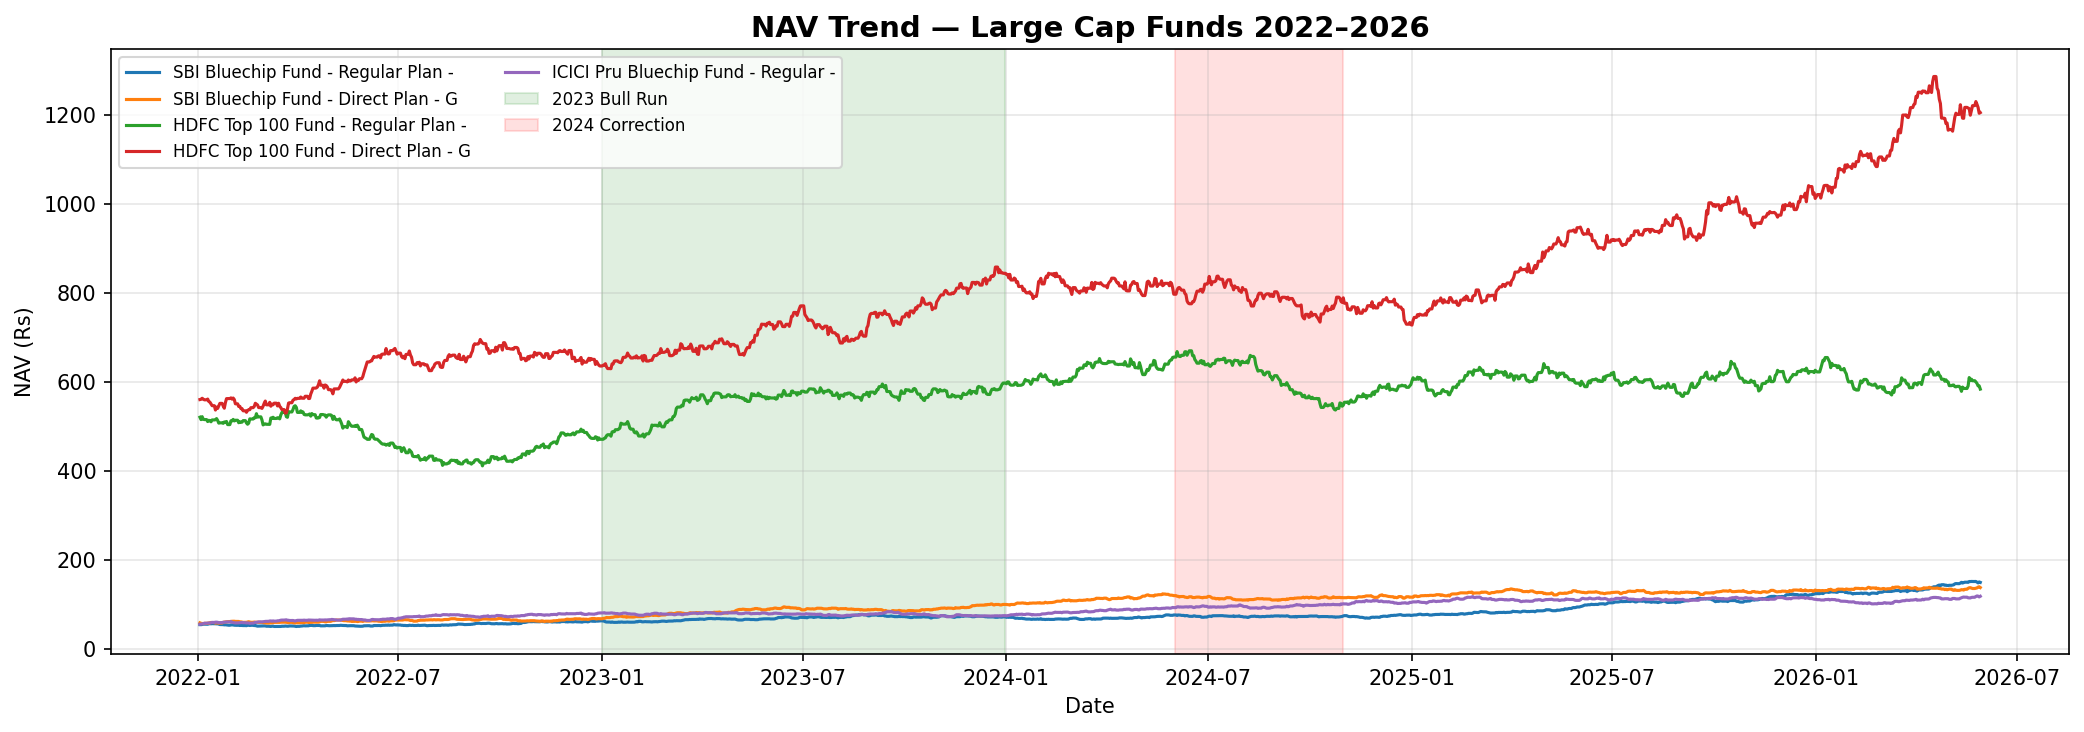
\includegraphics[width=\linewidth]{figures/chart1_nav_trend.png}
\caption{NAV trends for five large-cap schemes (2022--2026), with the 2023
bull run and 2024 correction periods highlighted.}
\label{fig:nav_trend}
\end{figure}

\subsection{AUM Concentration by Fund House}
Figure~\ref{fig:aum_growth} presents AUM by fund house across 2022--2025.
Aggregating scheme-level AUM from the performance dataset, the total
across all 40 schemes is approximately Rs.\ 10.44 lakh crore, with SBI
Mutual Fund, ICICI Prudential, and HDFC Mutual Fund among the largest
contributors.

\begin{figure}[h]
\centering
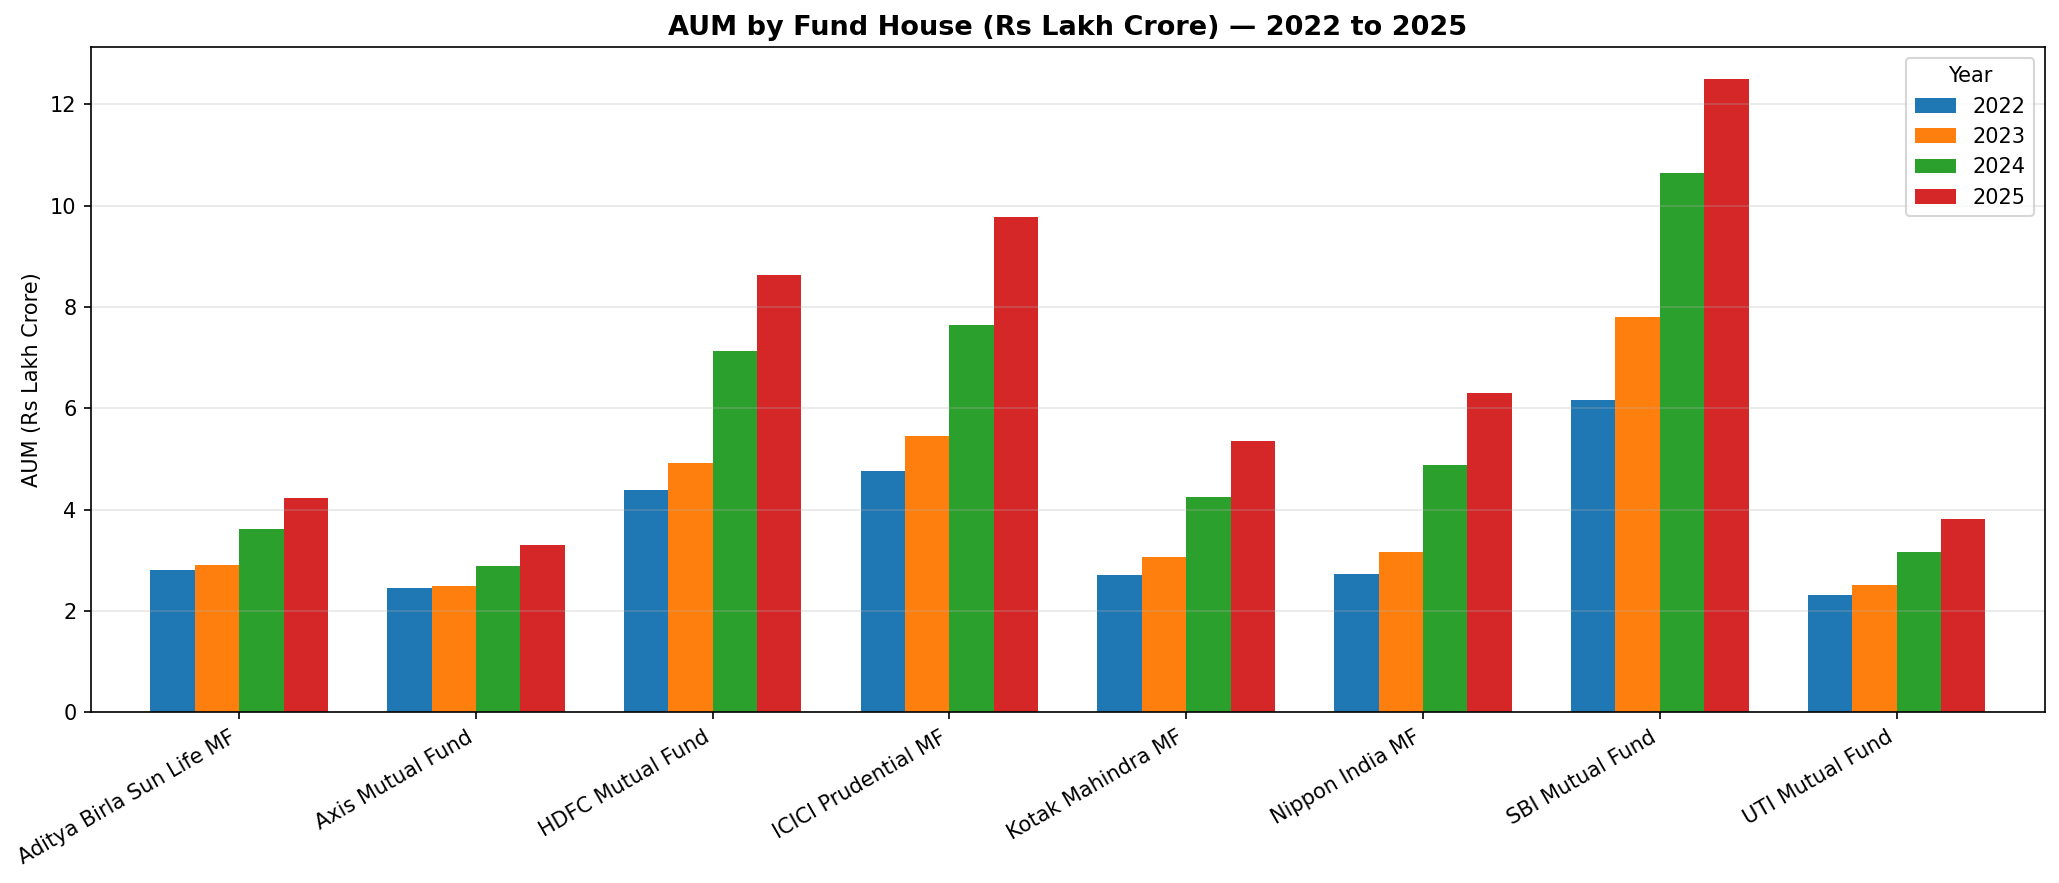
\includegraphics[width=\linewidth]{figures/chart2_aum_growth.png}
\caption{AUM by fund house (Rs.\ lakh crore), 2022--2025.}
\label{fig:aum_growth}
\end{figure}

\subsection{SIP Inflows and Folio Growth}
Monthly SIP inflows grew from Rs.\ 11{,}517 crore in January 2022 to an
all-time high of Rs.\ 31{,}002 crore in December 2025
(Figure~\ref{fig:sip}), an increase of roughly 169\% over the four-year
window. Over the same period, industry folio counts nearly doubled, from
13.26 crore to 26.12 crore (Figure~\ref{fig:folio}).

\begin{figure}[h]
\centering
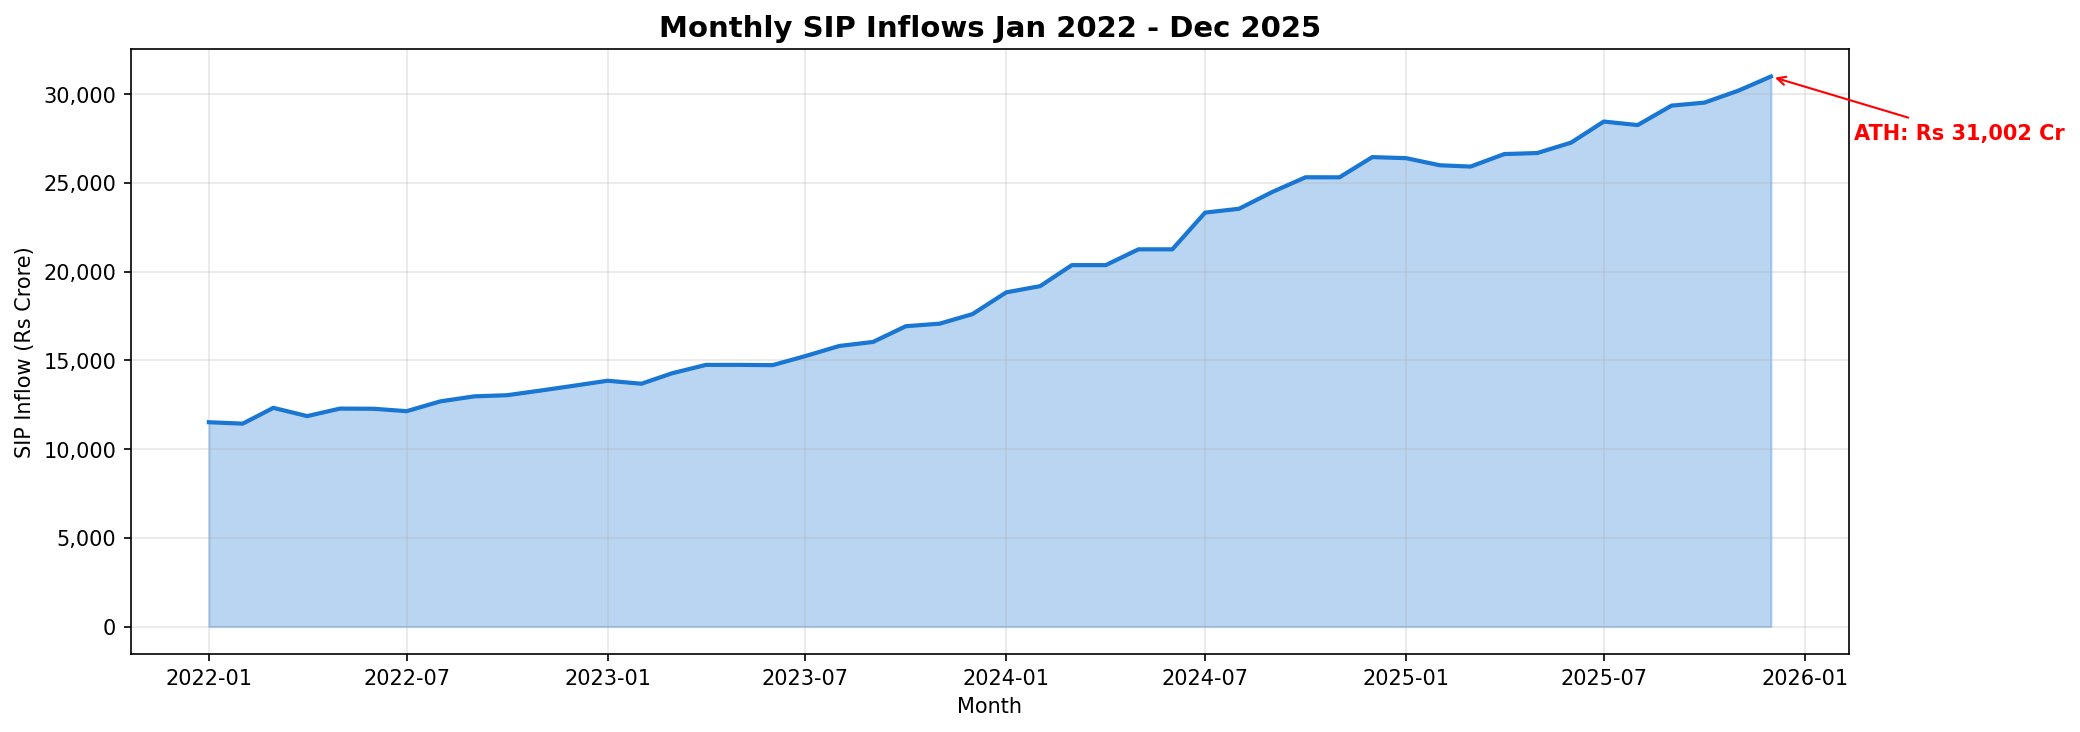
\includegraphics[width=\linewidth]{figures/chart3_sip_inflow.png}
\caption{Monthly SIP inflows (Rs.\ crore), January 2022 -- December 2025,
with the all-time-high month annotated.}
\label{fig:sip}
\end{figure}

\begin{figure}[h]
\centering
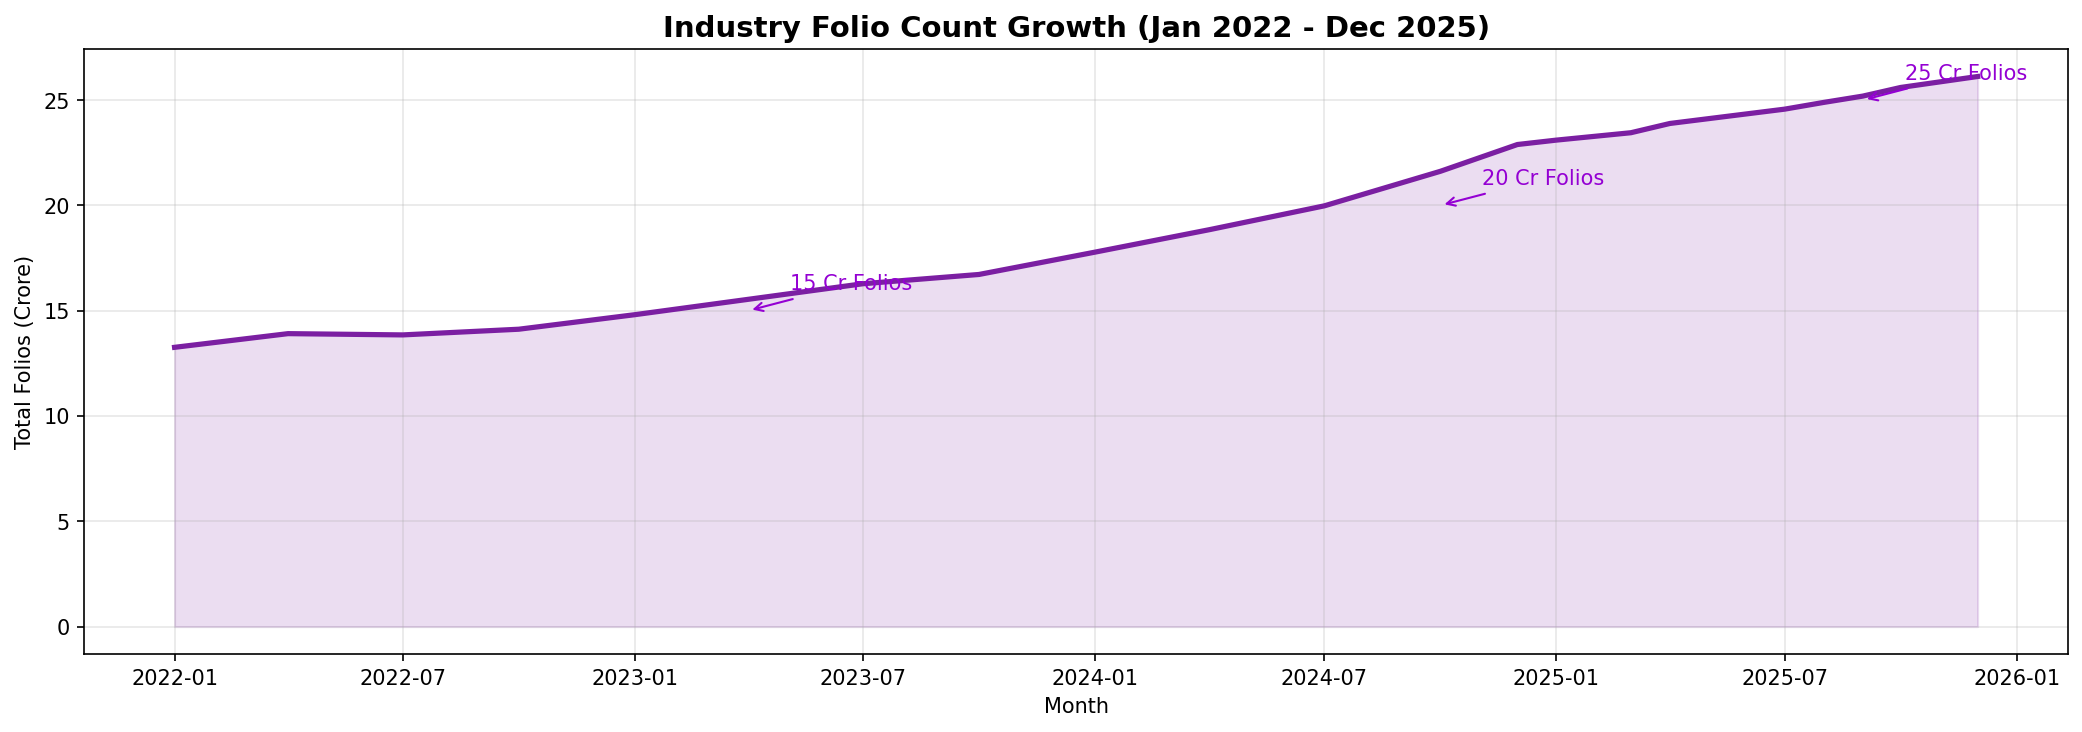
\includegraphics[width=\linewidth]{figures/chart7_folio_growth.png}
\caption{Industry folio count growth (crore accounts), Jan 2022 -- Dec 2025.}
\label{fig:folio}
\end{figure}

\subsection{Category Inflow Patterns}
The category-level inflow heatmap (Figure~\ref{fig:cat_heatmap}) shows
inflow intensity varying substantially across equity and debt categories
over time, with equity-oriented categories generally showing stronger and
more sustained positive net inflows than debt categories during the
2023--2025 window.

\begin{figure}[h]
\centering
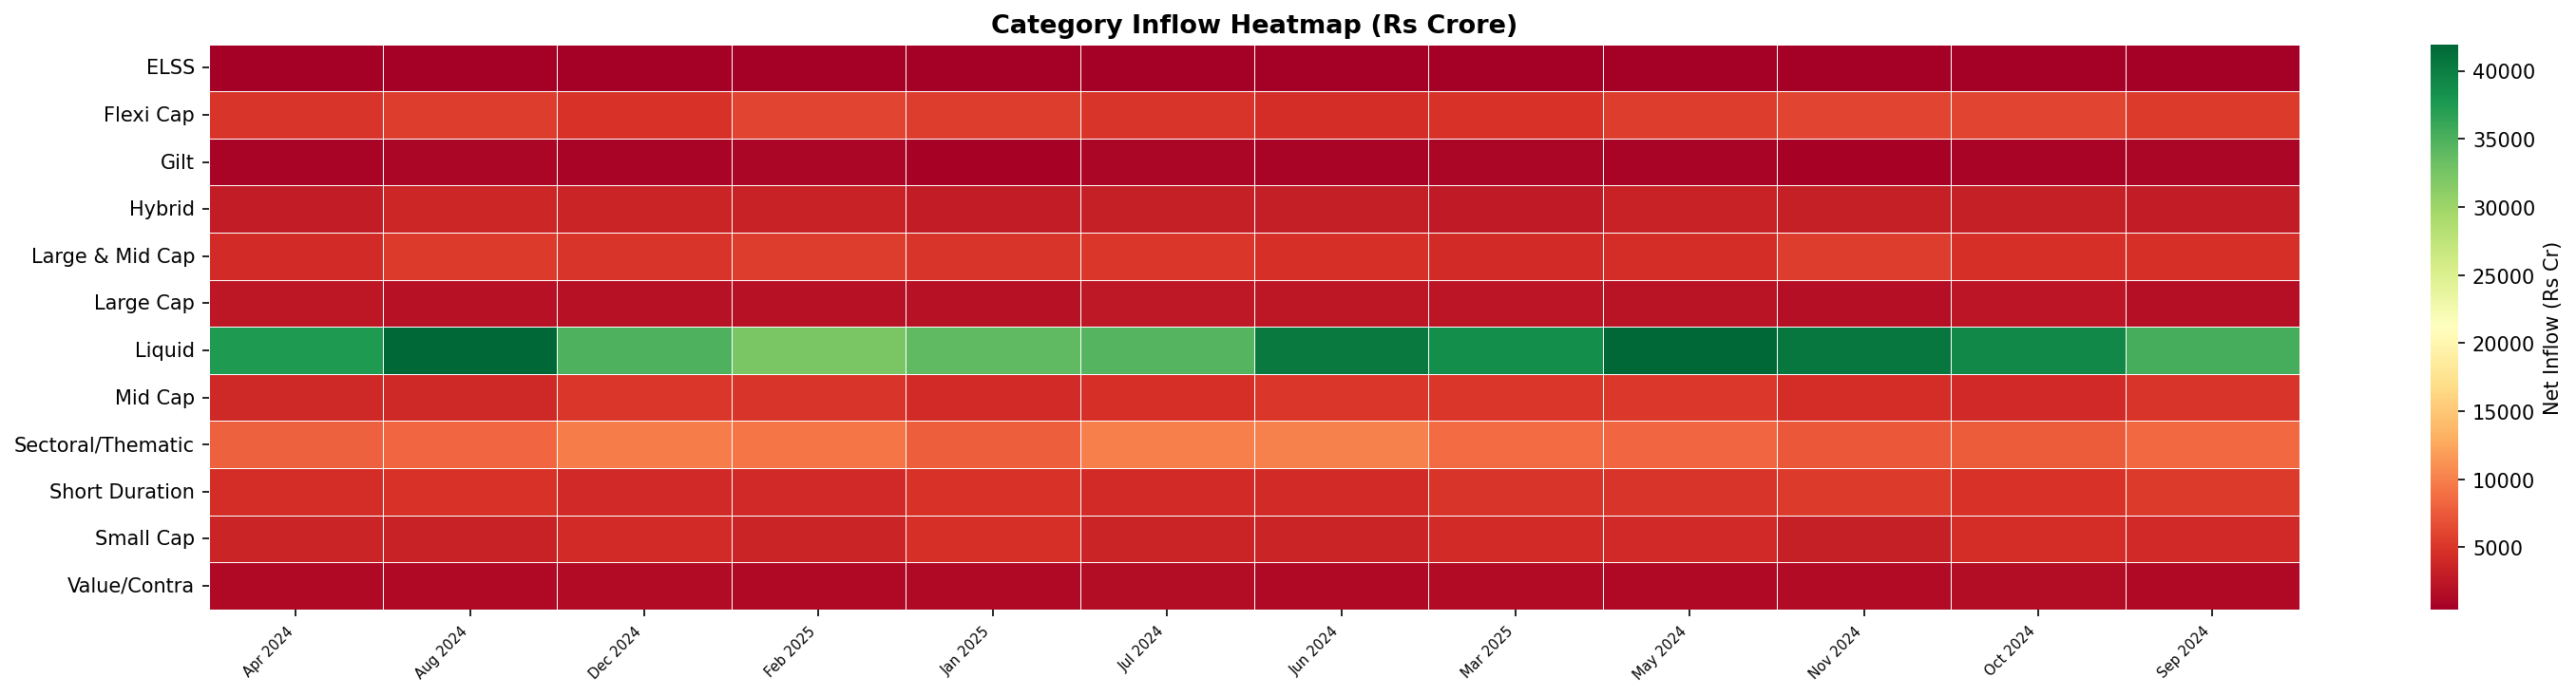
\includegraphics[width=\linewidth]{figures/chart4_category_heatmap.png}
\caption{Net inflow by category and month (Rs.\ crore); green indicates
positive net inflow, red indicates outflow.}
\label{fig:cat_heatmap}
\end{figure}

\subsection{Sector Allocation and Return Correlation}
Aggregating portfolio holdings across all equity schemes
(Figure~\ref{fig:sector_alloc}), Financials and Information Technology
represent the two largest sector exposures, consistent with the
composition of major Indian equity benchmarks. The pairwise return
correlation matrix for 12 representative funds (Figure~\ref{fig:corr})
shows correlations in the 0.7--0.95 range among large-cap and flexi-cap
funds, indicating limited diversification benefit when combining funds from
similar sub-categories.

\begin{figure}[h]
\centering
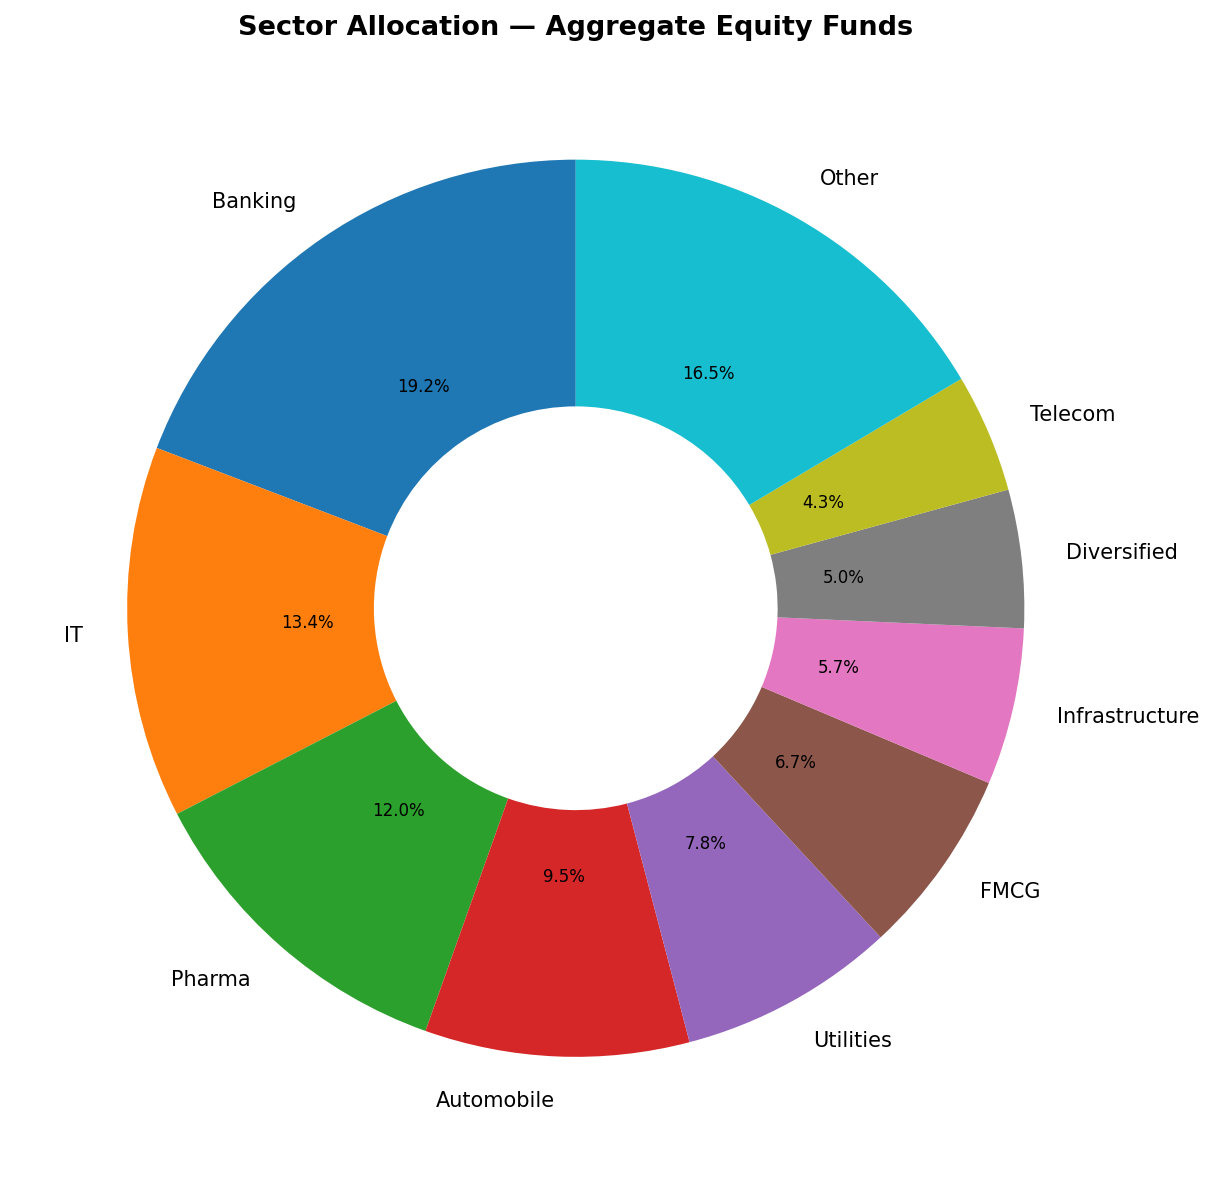
\includegraphics[width=\linewidth]{figures/chart9_sector_allocation.png}
\caption{Aggregate sector allocation across equity scheme holdings.}
\label{fig:sector_alloc}
\end{figure}

\begin{figure}[h]
\centering
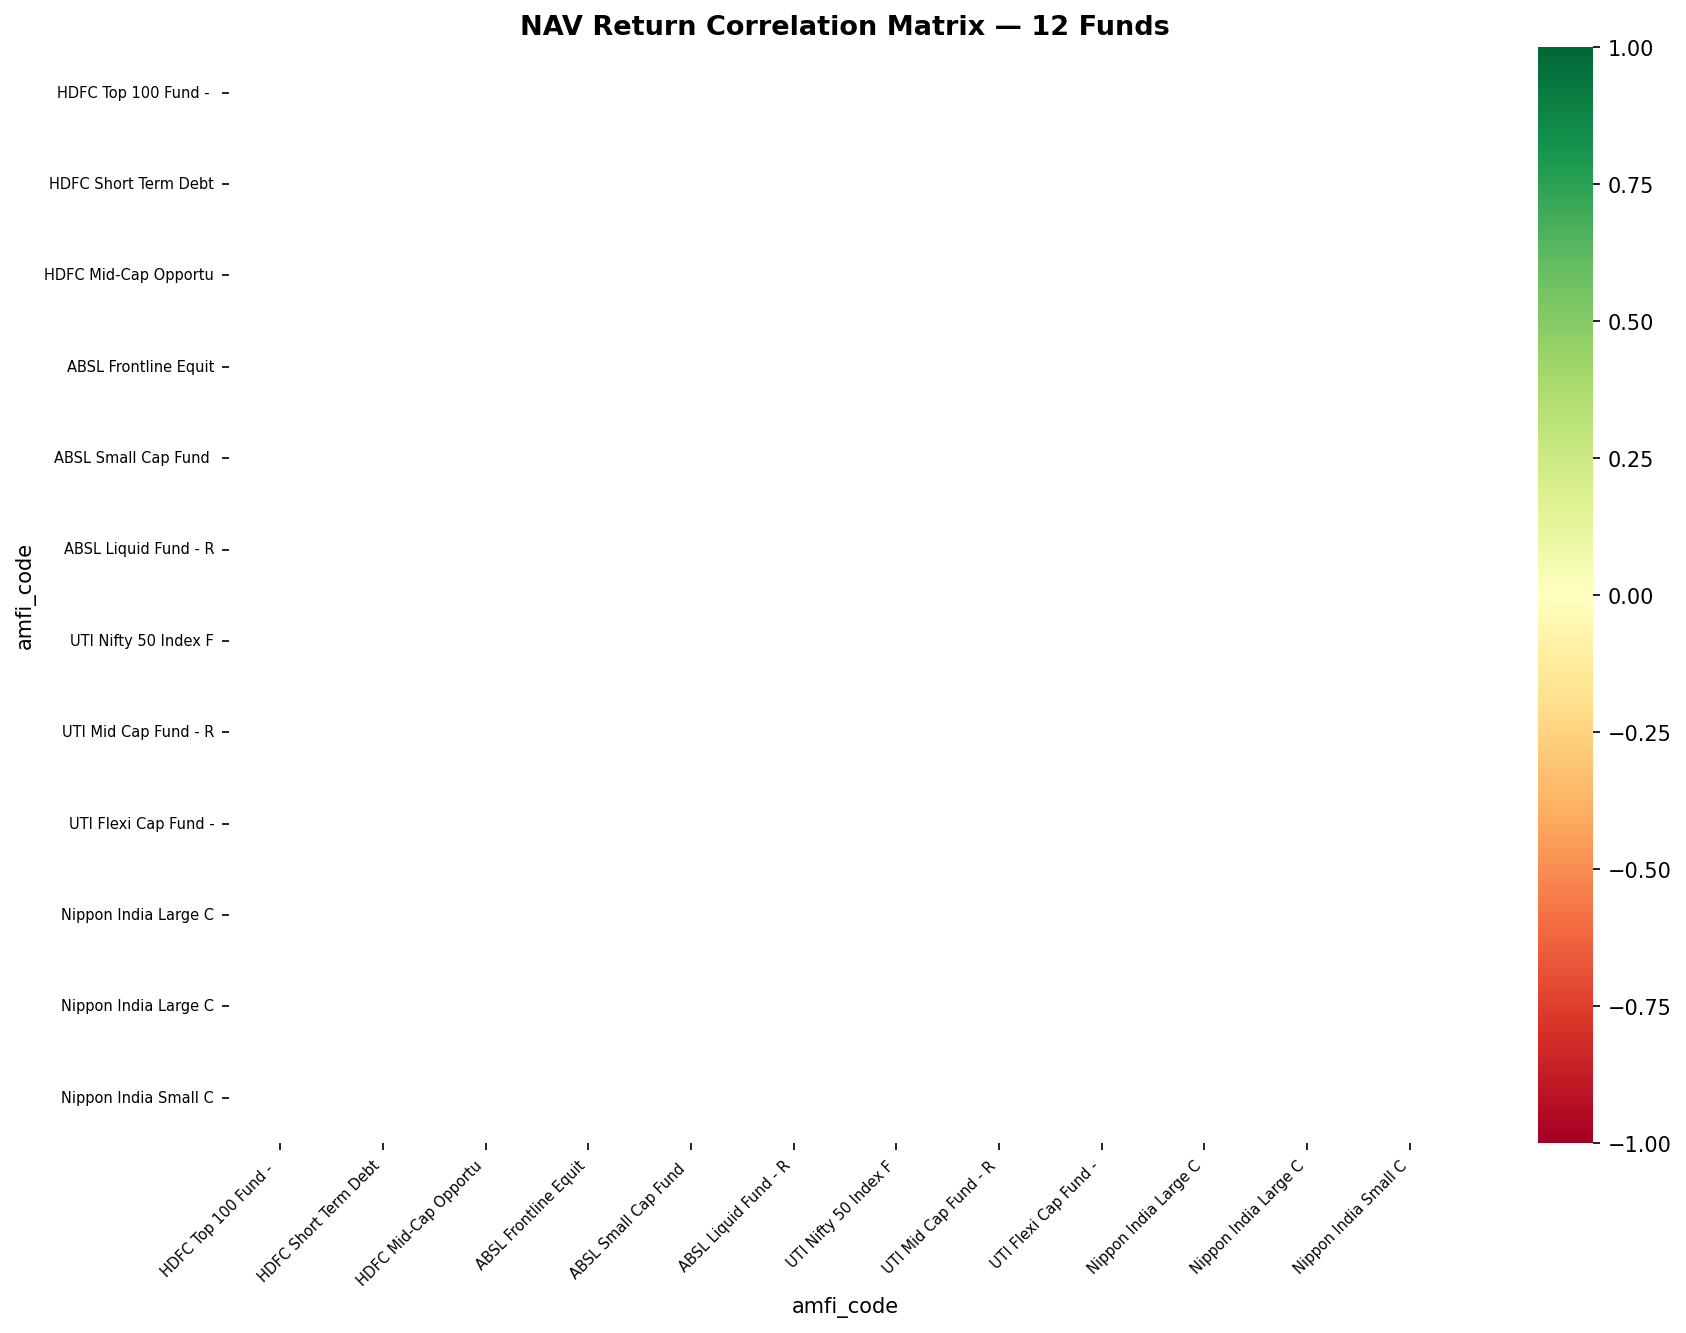
\includegraphics[width=\linewidth]{figures/chart8_correlation_matrix.png}
\caption{Pairwise correlation matrix of daily returns for 12 representative
schemes.}
\label{fig:corr}
\end{figure}

\section{Performance Analytics}

\subsection{Methodology}
For each scheme $i$, the daily return is defined as
\begin{equation}
r_{i,t} = \frac{\text{NAV}_{i,t}}{\text{NAV}_{i,t-1}} - 1.
\end{equation}
CAGR over $n$ years is computed as
\begin{equation}
\text{CAGR}_{i} = \left(\frac{\text{NAV}_{i,\text{end}}}{\text{NAV}_{i,\text{start}}}\right)^{1/n} - 1.
\end{equation}
The Sharpe and Sortino ratios use a risk-free rate $R_f = 6.5\%$ (a proxy
for the RBI repo rate):
\begin{equation}
\text{Sharpe}_i = \frac{\bar{r}_i - R_f^{d}}{\sigma_i}\sqrt{252}, \qquad
\text{Sortino}_i = \frac{\bar{r}_i - R_f^{d}}{\sigma_i^{-}}\sqrt{252},
\end{equation}
where $\sigma_i^{-}$ is the standard deviation of negative excess-return
days only. Jensen's alpha and beta are estimated via ordinary least squares
regression of fund returns on NIFTY 100 returns,
$r_{i,t} = \alpha_i + \beta_i r_{m,t} + \varepsilon_t$, with
$\alpha^{\text{ann}}_i = \alpha_i \times 252$. Maximum drawdown is
$\text{MDD}_i = \min_t \left( \text{NAV}_{i,t}/\max_{s\le t}\text{NAV}_{i,s} - 1\right)$.

\subsection{Composite Fund Scorecard}
A composite score on a 0--100 scale was constructed for each scheme as a
weighted combination of percentile ranks:
\begin{equation}
\begin{aligned}
\text{Score}_i = \;& 0.30 \cdot \text{rank}(\text{CAGR}_{3y,i}) + 0.25 \cdot \text{rank}(\text{Sharpe}_i) \\
& + 0.20 \cdot \text{rank}(\alpha^{\text{ann}}_i) + 0.15 \cdot \text{rank}^{-1}(\text{ExpRatio}_i) \\
& + 0.10 \cdot \text{rank}^{-1}(\text{MDD}_i),
\end{aligned}
\end{equation}
where $\text{rank}^{-1}$ denotes an inverted percentile rank (lower expense
ratio and shallower drawdown score higher). Table~\ref{tab:scorecard}
reports the top five schemes by composite score.

\begin{table}[h]
\centering
\small
\caption{Top 5 schemes by composite Fund Scorecard}
\label{tab:scorecard}
\begin{tabular}{@{}lrrr@{}}
\toprule
\textbf{Scheme} & \textbf{CAGR3y} & \textbf{Sharpe} & \textbf{Score} \\
\midrule
ICICI Pru Midcap          & 31.78\% & 0.883 & 84.50 \\
Axis Midcap                & 35.11\% & 0.731 & 81.38 \\
HDFC Mid-Cap Opp.           & 32.44\% & 0.808 & 79.88 \\
Mirae Asset Large Cap       & 34.00\% & 1.068 & 79.38 \\
Kotak Flexicap              & 29.58\% & 0.966 & 77.62 \\
\bottomrule
\end{tabular}
\end{table}

\begin{figure}[h]
\centering
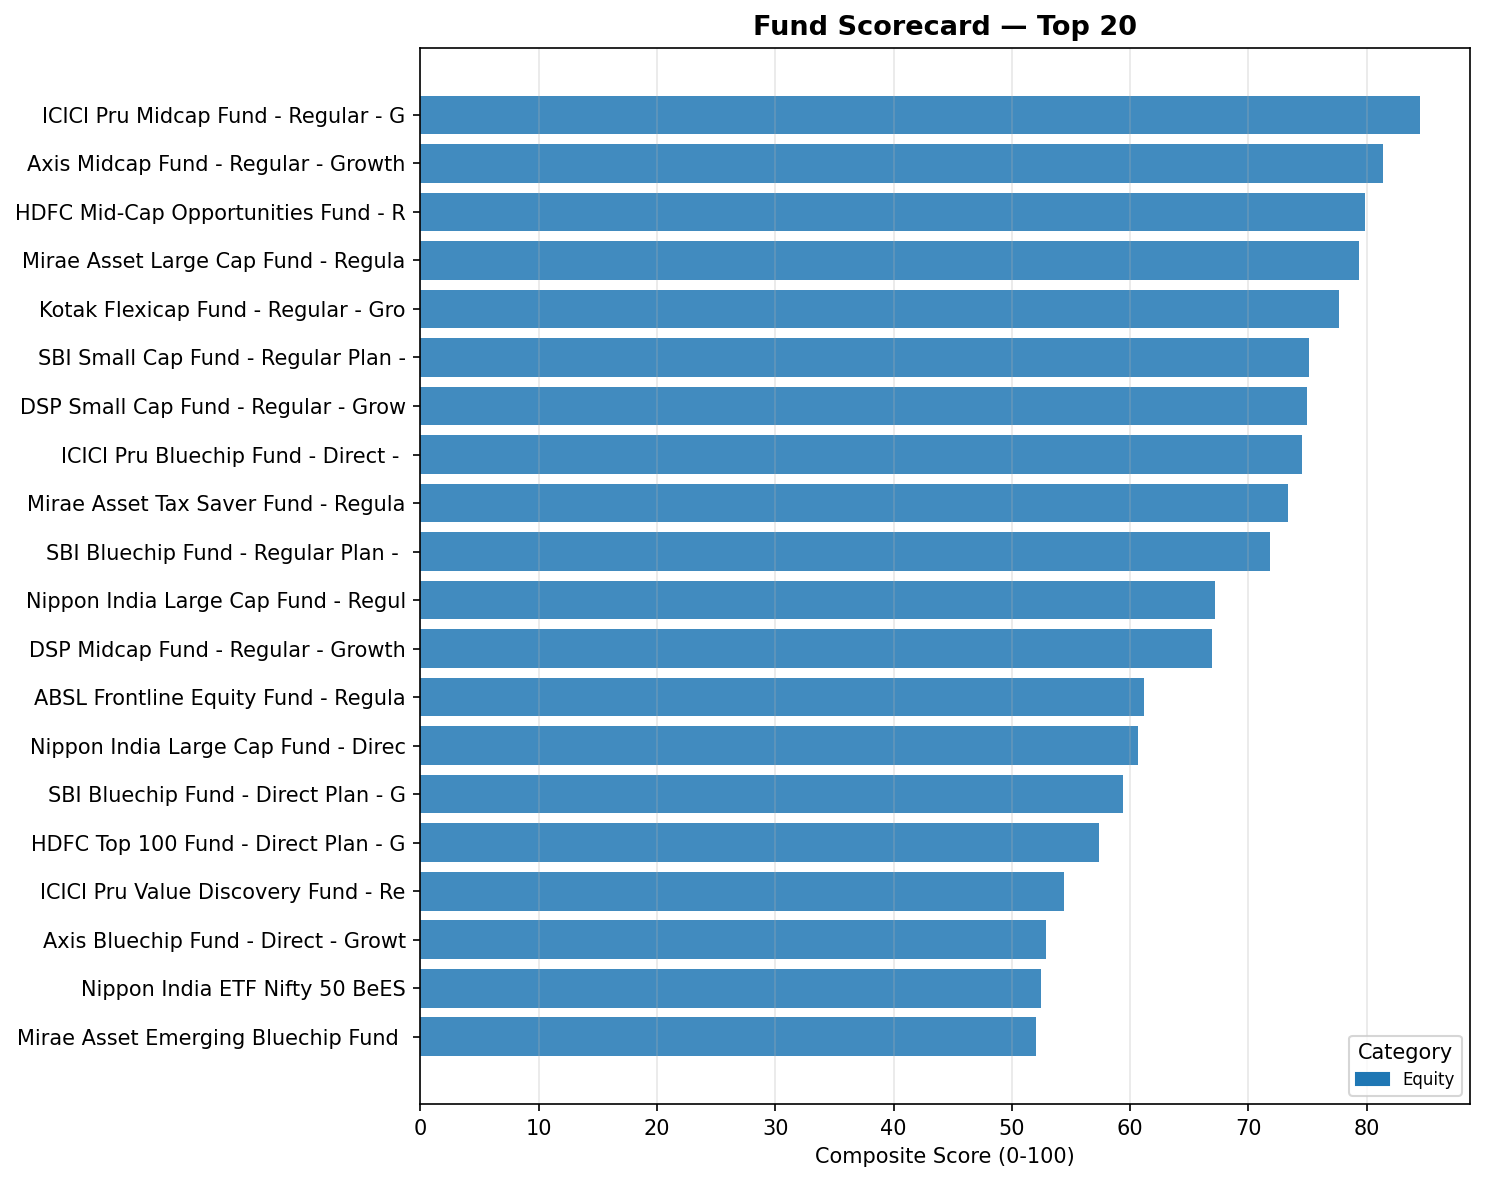
\includegraphics[width=\linewidth]{figures/chart_fund_scorecard.png}
\caption{Top 20 schemes ranked by composite Fund Scorecard, coloured by
category.}
\label{fig:scorecard}
\end{figure}

Mid-cap equity funds dominate the top of the scorecard, reflecting strong
3-year CAGR figures (29--35\%) combined with competitive Sharpe ratios. The
schemes with the highest annualised alpha against NIFTY 100 were SBI Small
Cap (+30.34\%), DSP Small Cap (+30.06\%), and ICICI Prudential Midcap
(+29.26\%), each exhibiting betas close to zero, suggesting return drivers
largely independent of the large-cap benchmark over the sample window.

\subsection{Drawdown Risk}
The deepest maximum drawdowns were observed in small-cap schemes: SBI Small
Cap Direct Plan ($-52.6\%$), Axis Small Cap ($-51.7\%$), and ABSL Small Cap
($-35.5\%$), all with trough dates falling in late 2025 / mid-2026,
consistent with elevated small-cap volatility relative to large-cap and
flexi-cap peers.

\subsection{Benchmark Comparison}
Figure~\ref{fig:benchmark} compares the top five scorecard funds against
NIFTY 50 and NIFTY 100 on a rebased (=100) cumulative basis. All five funds
outperformed both benchmarks over the sample window, with the tracking
error for the top performers in the range of moderate single digits,
reflecting active deviation from benchmark composition consistent with
mid-cap and flexi-cap mandates.

\begin{figure}[h]
\centering
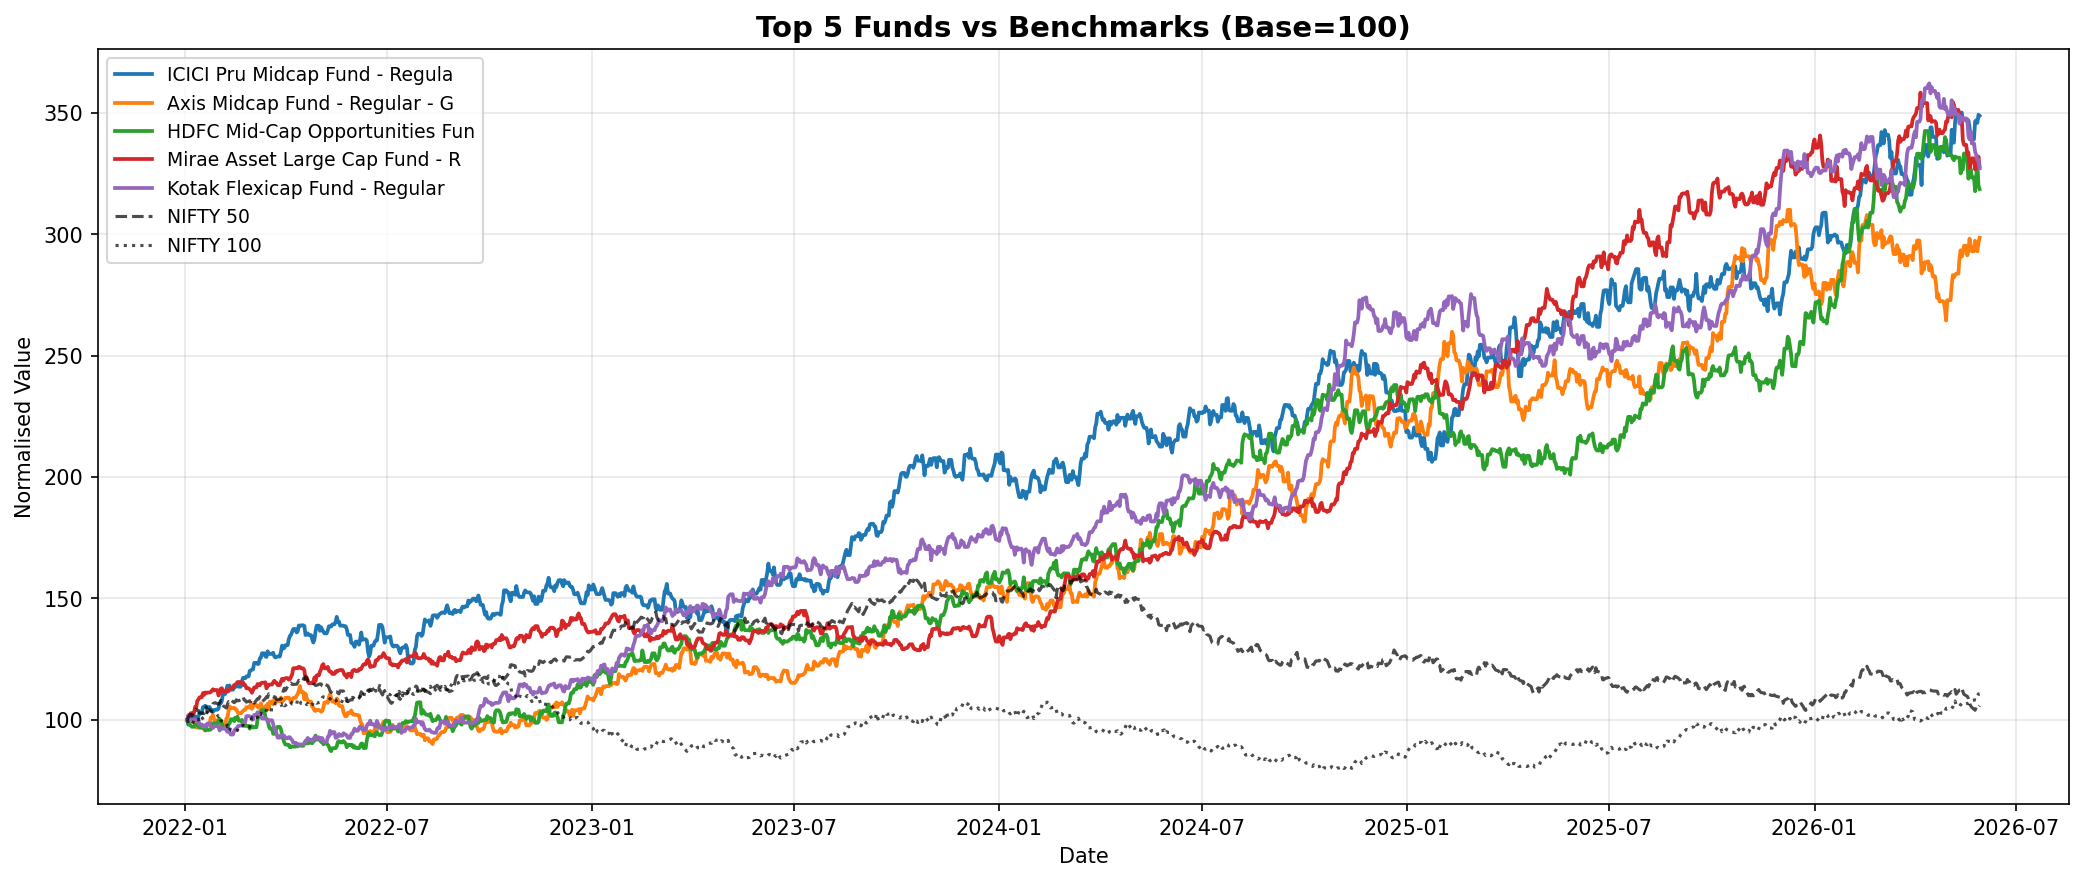
\includegraphics[width=\linewidth]{figures/chart_benchmark_comparison.png}
\caption{Top 5 scorecard funds vs.\ NIFTY 50 and NIFTY 100 (rebased to 100).}
\label{fig:benchmark}
\end{figure}

\section{Advanced Risk and Behavioural Analytics}

\subsection{Value-at-Risk and Conditional VaR}
Historical 95\% VaR was computed as the 5th percentile of the daily return
distribution, with CVaR as the mean of returns falling below this
threshold. Figure~\ref{fig:var} shows the 15 riskiest schemes by
VaR$_{95}$. The highest-risk schemes are exclusively small-cap funds: ABSL
Small Cap ($\text{VaR}_{95}=-2.39\%$, $\text{CVaR}_{95}=-3.03\%$), Axis
Small Cap ($-2.33\%$ / $-2.97\%$), and SBI Small Cap Direct
($-2.32\%$ / $-3.02\%$), each with annualised volatility around 21\%.

\begin{figure}[h]
\centering
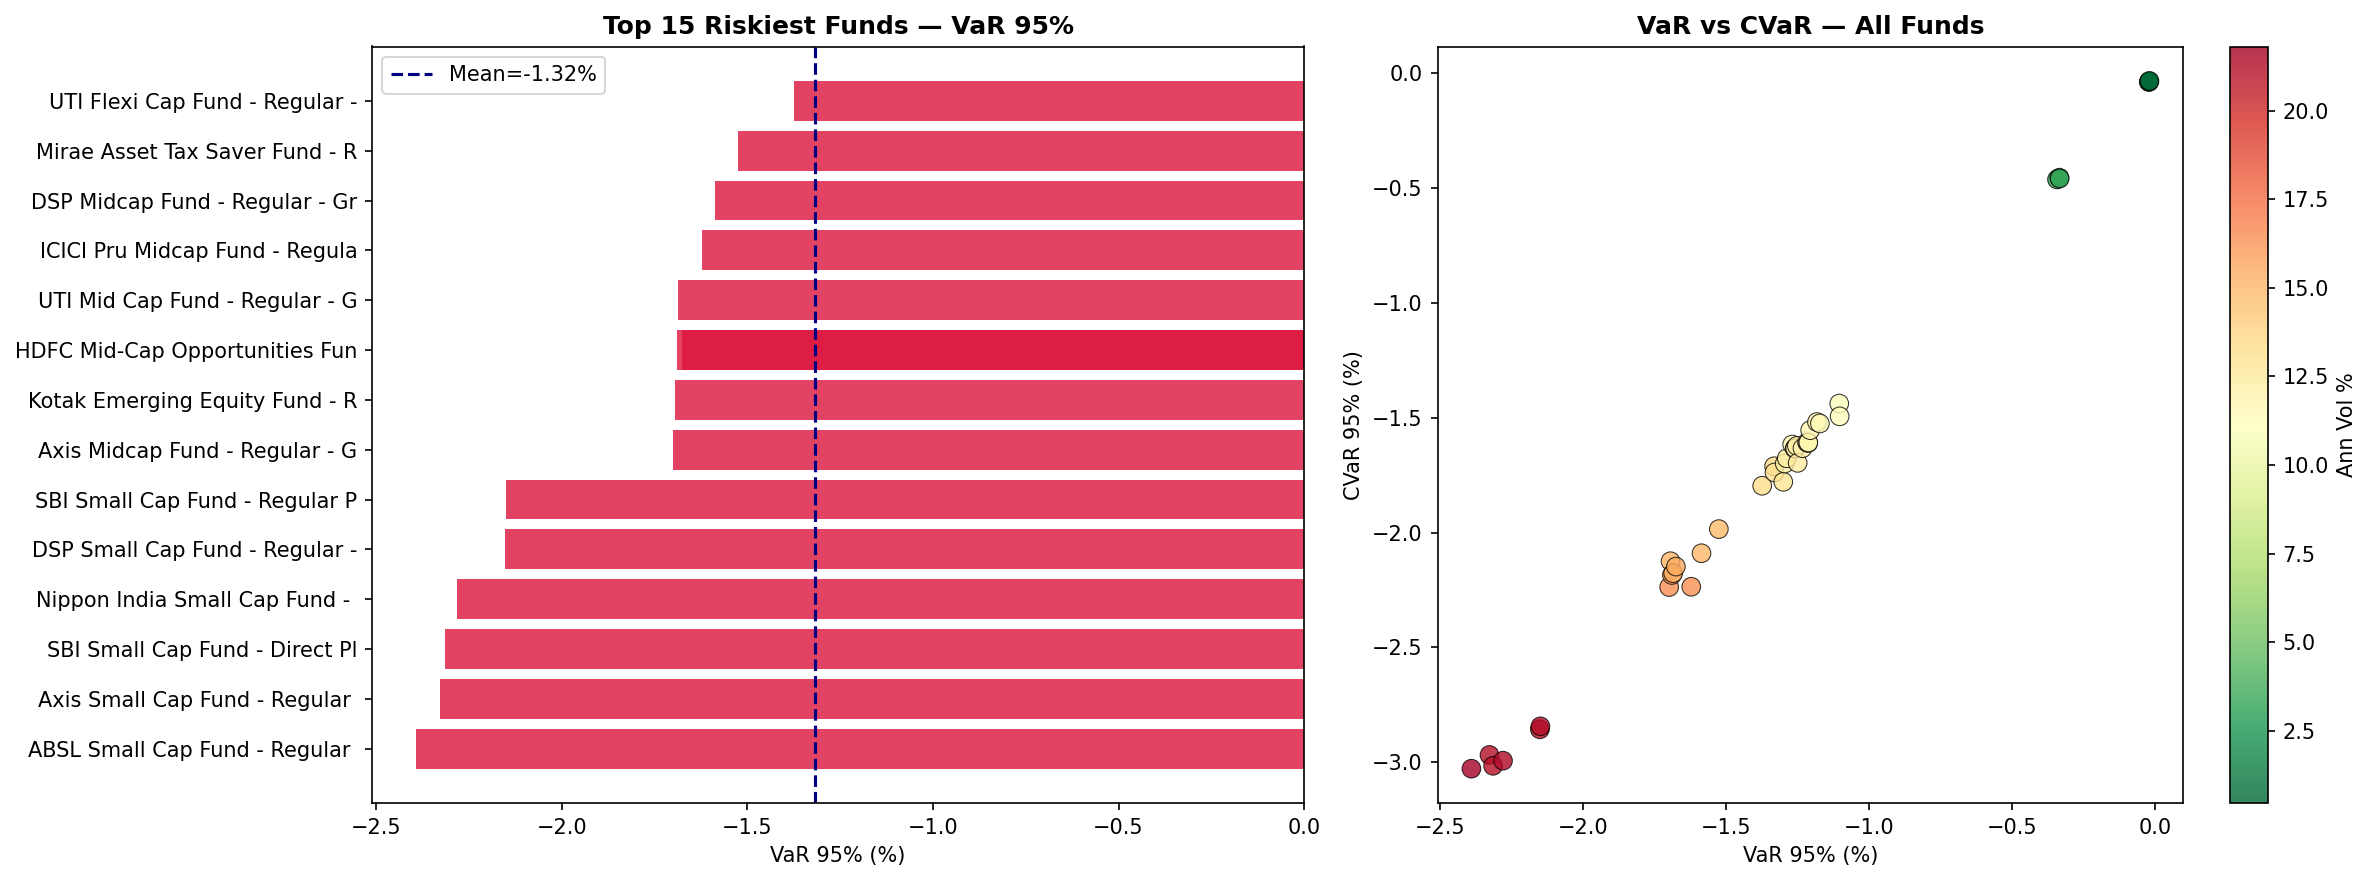
\includegraphics[width=\linewidth]{figures/chart_var_cvar.png}
\caption{Left: Top 15 schemes by VaR$_{95}$. Right: VaR vs.\ CVaR scatter
coloured by annualised volatility.}
\label{fig:var}
\end{figure}

\subsection{Rolling 90-Day Sharpe Ratio}
The rolling 90-day Sharpe ratio for the five most data-complete schemes
(Figure~\ref{fig:rolling_sharpe}) confirms the regime shifts visible in the
NAV trend chart: Sharpe ratios compress toward zero or turn negative during
the 2024 correction window before recovering through 2025, illustrating
time-varying risk-adjusted performance that a single full-sample Sharpe
ratio would obscure.

\begin{figure}[h]
\centering
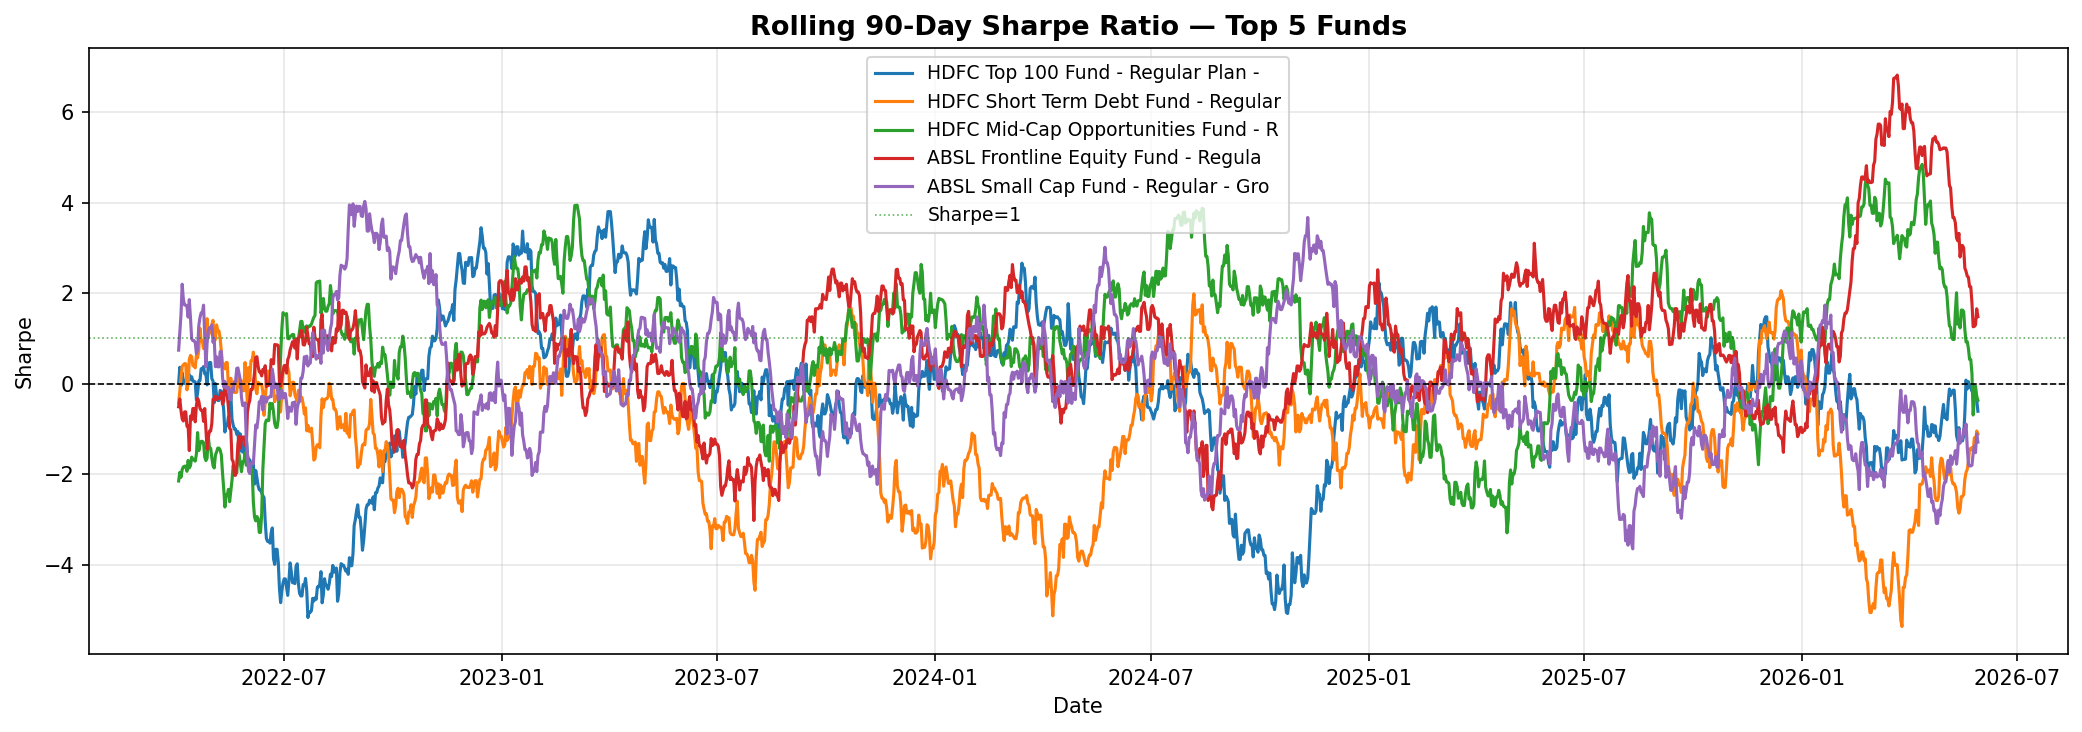
\includegraphics[width=\linewidth]{figures/rolling_sharpe_chart.png}
\caption{Rolling 90-day Sharpe ratio for the five schemes with the longest
NAV history.}
\label{fig:rolling_sharpe}
\end{figure}

\subsection{Investor Cohort Analysis}
Investors were grouped by the calendar year of their first recorded
transaction. The resulting cohorts (Table~\ref{tab:cohort}) show that the
2024 cohort accounts for the overwhelming majority of investors (4{,}803)
and transaction volume (32{,}499 transactions, totalling approximately Rs.\
349 crore invested), with an average SIP ticket size of roughly Rs.\
1{,}074. The smaller 2025 cohort shows a marginally higher average SIP
amount (Rs.\ 1{,}092), and both cohorts' top fund preference includes
passive (Nifty 50 Index) and small-cap active strategies.

\begin{table}[h]
\centering
\small
\caption{Investor cohort summary by first-transaction year}
\label{tab:cohort}
\begin{tabular}{@{}lrrr@{}}
\toprule
\textbf{Cohort} & \textbf{Investors} & \textbf{Txns} & \textbf{Avg.\ SIP (Rs.)} \\
\midrule
2024 & 4{,}803 & 32{,}499 & 1{,}074.23 \\
2025 & 197    & 279     & 1{,}091.59 \\
\bottomrule
\end{tabular}
\end{table}

\begin{figure}[h]
\centering
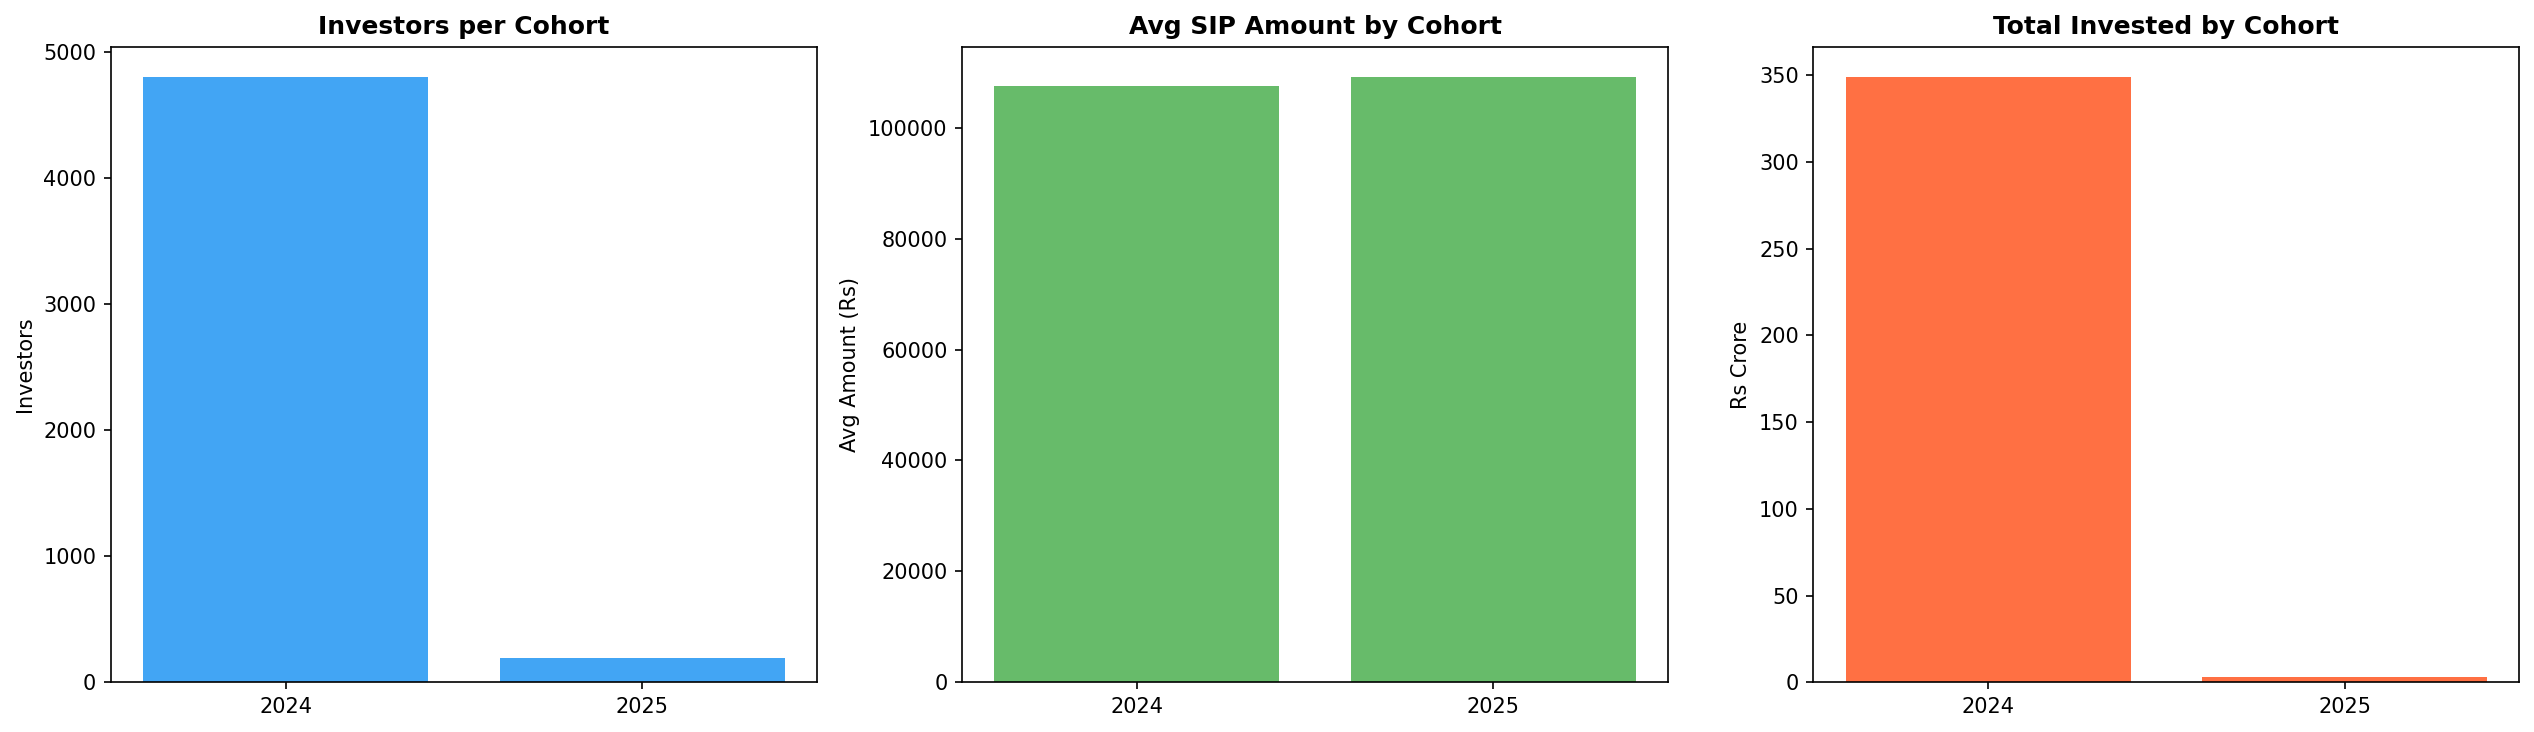
\includegraphics[width=\linewidth]{figures/chart_cohort_analysis.png}
\caption{Investor count, average SIP amount, and total invested by
first-transaction-year cohort.}
\label{fig:cohort}
\end{figure}

\subsection{SIP Continuity}
Among investors with six or more SIP transactions, the average gap between
consecutive SIPs was computed; investors with an average gap exceeding 35
days were flagged as \textit{at-risk} of SIP discontinuation. Of 1{,}362
qualifying investors, a substantial majority were flagged as at-risk under
this threshold, indicating that irregular SIP cadence is widespread in the
sample and represents a meaningful retention-management opportunity for
fund houses and distributors.

\subsection{Sector Concentration (HHI)}
Portfolio concentration was measured via the Herfindahl--Hirschman Index,
$\text{HHI}_i = \sum_k w_{i,k}^2$, over sector weights $w_{i,k}$ for each
equity scheme $i$. Figure~\ref{fig:hhi} shows that the Axis Bluechip Fund
and ABSL Small Cap Fund exhibit the highest concentration (HHI $\approx$
2{,}000--2{,}065, \textit{Moderate} band), while Nippon India Small Cap and
both SBI Bluechip variants show the lowest concentration (HHI $\approx$
1{,}073--1{,}084, \textit{Low} band). No scheme in the sample crossed the
2{,}500 \textit{High} concentration threshold, suggesting reasonably
diversified sector exposure across the fund universe relative to
conventional concentration benchmarks.

\begin{figure}[h]
\centering
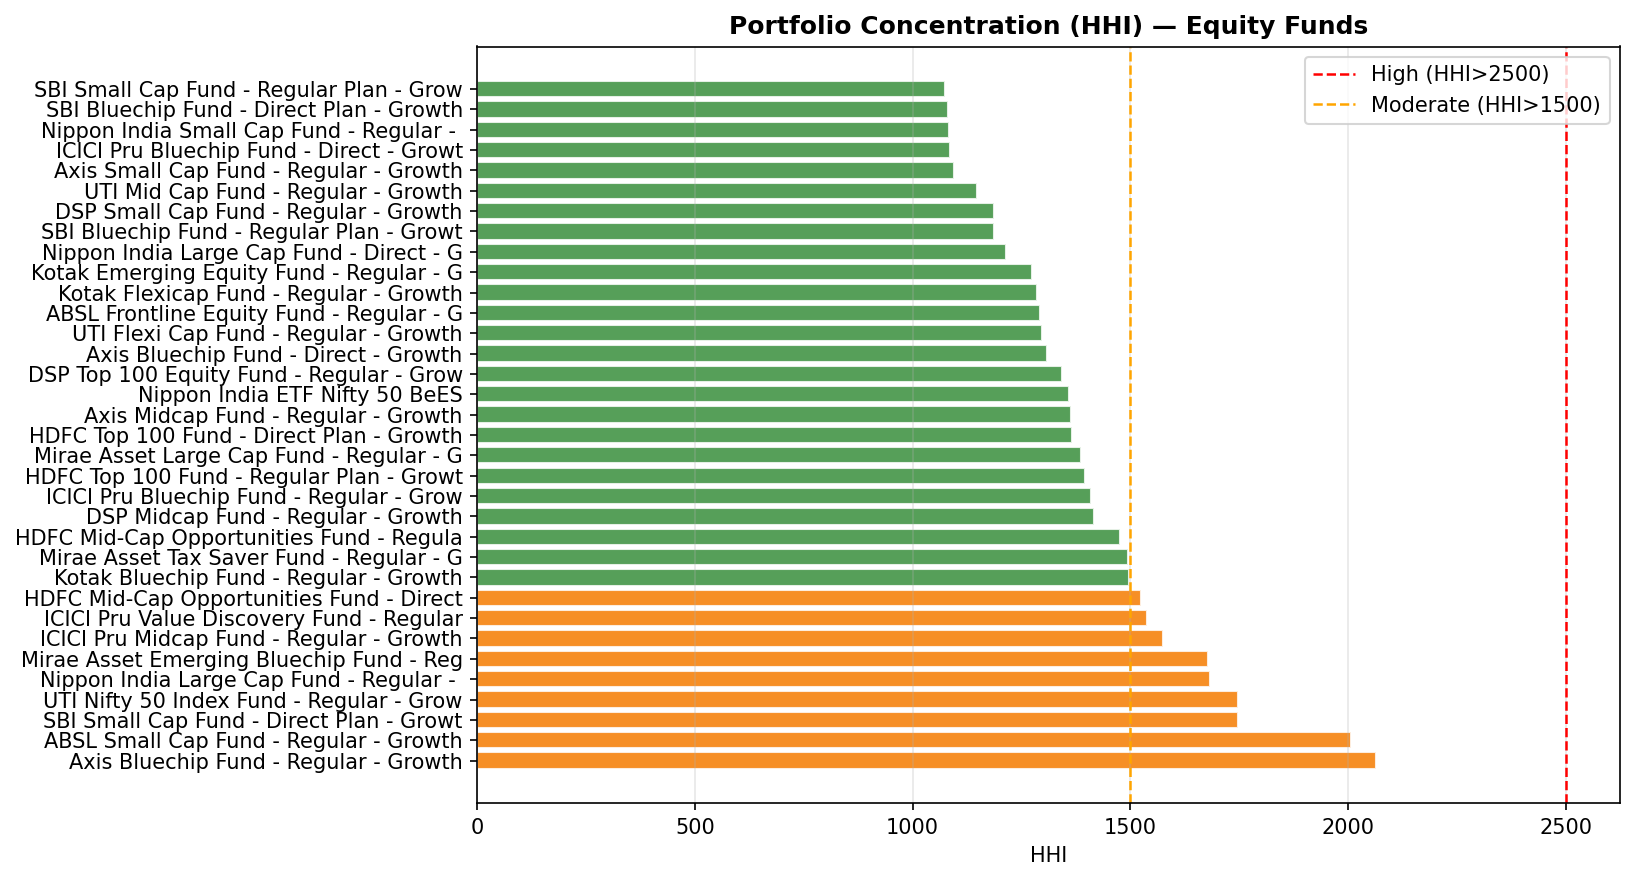
\includegraphics[width=\linewidth]{figures/chart_sector_hhi.png}
\caption{Herfindahl--Hirschman Index by equity scheme, with Moderate
(HHI$>$1500) and High (HHI$>$2500) thresholds annotated.}
\label{fig:hhi}
\end{figure}

\subsection{Risk-Appetite-Based Fund Recommender}
A rule-based recommender filters the Fund Scorecard by an investor's stated
risk appetite -- Low, Moderate, or High -- mapped onto the dataset's
\texttt{risk\_grade} field (e.g.\ Moderate maps to \{\textit{Moderate},
\textit{Moderately High}\}), and returns the top three schemes by Sharpe
ratio within that band. For a \textit{Moderate} risk appetite, the
recommender returns Mirae Asset Large Cap Fund (Sharpe $=1.068$), Kotak
Flexicap Fund (Sharpe $=0.966$), and SBI Bluechip Fund (Sharpe $=0.861$),
illustrating how the composite scorecard can be operationalised for
investor-facing recommendations.

\section{Risk--Return Trade-off Summary}
Figure~\ref{fig:risk_return} consolidates the risk and return dimensions
across all 40 schemes, plotting annualised standard deviation against 3-year
CAGR with bubble size proportional to AUM and colour representing the
Sharpe ratio. The plot visually corroborates the category-level findings:
small-cap schemes occupy the high-risk / high-return region with generally
lower Sharpe ratios, while large-cap and flexi-cap schemes cluster in a
more favourable lower-risk region with comparatively higher Sharpe ratios,
consistent with their dominance of the composite scorecard.

\begin{figure}[h]
\centering
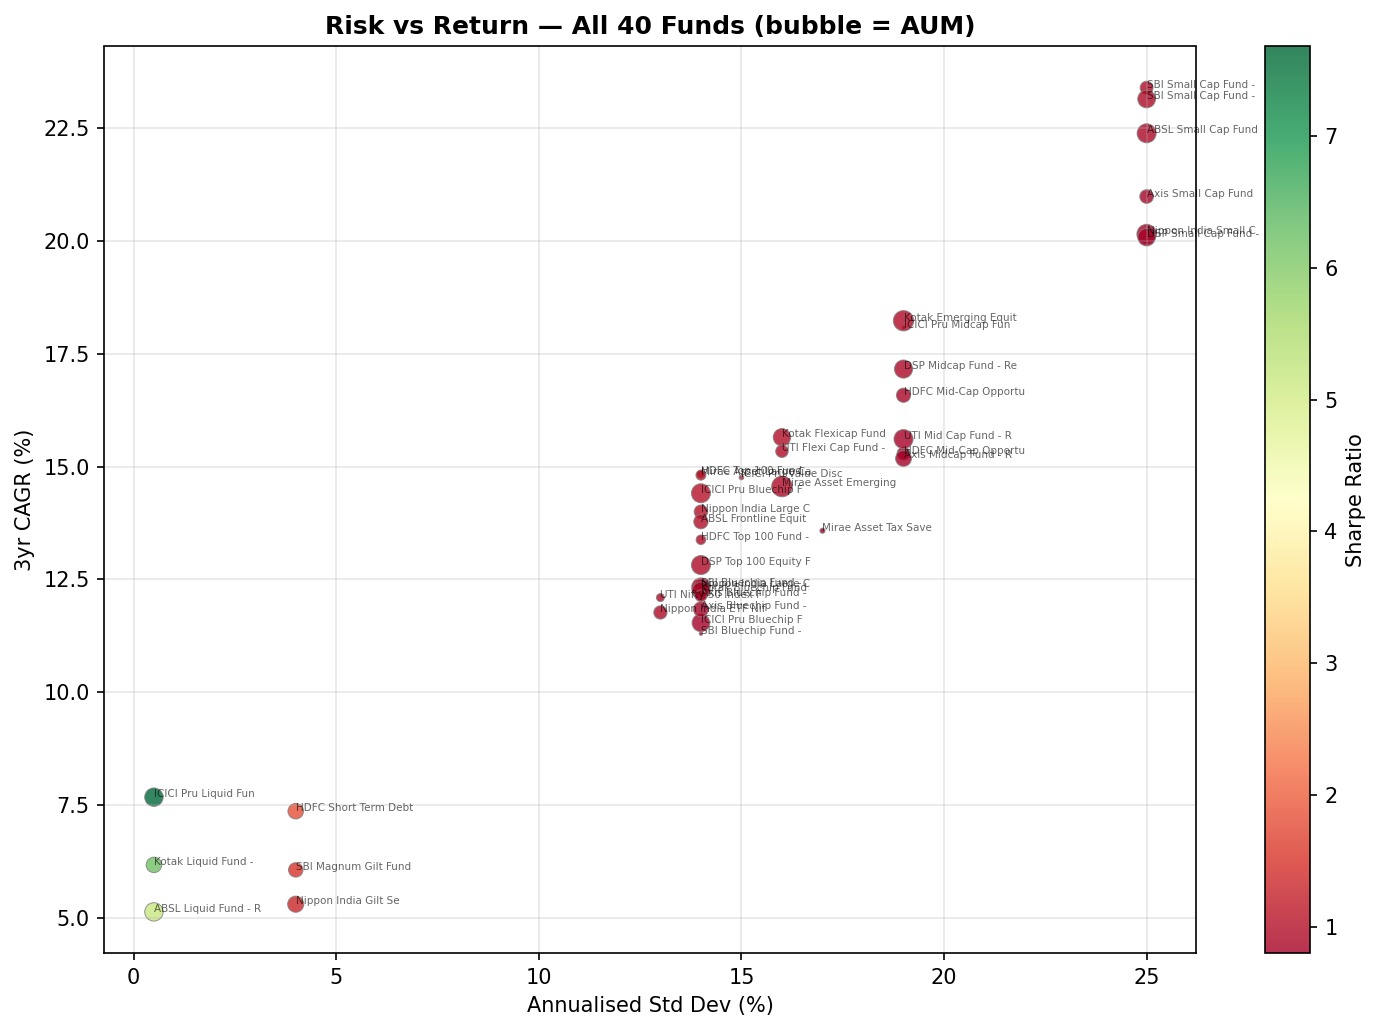
\includegraphics[width=\linewidth]{figures/chart10_risk_return.png}
\caption{Risk (annualised std.\ dev.) vs.\ 3-year CAGR across all 40
schemes; bubble size = AUM, colour = Sharpe ratio.}
\label{fig:risk_return}
\end{figure}

\section{Discussion}
Three themes emerge from this analysis. First, the performance--risk
trade-off is strongly category-driven: mid-cap and flexi-cap funds achieve
the best risk-adjusted returns in the sample, while small-cap funds, despite
occasionally posting the highest raw alpha, carry disproportionately higher
tail risk (VaR$_{95}$ around $-2.3\%$ daily and drawdowns exceeding
$-50\%$). Second, industry growth metrics -- SIP inflows nearly tripling and
folio counts doubling over four years -- indicate sustained retail
participation, but the SIP continuity analysis suggests that a large share
of active SIP investors exhibit irregular contribution patterns, which has
direct implications for AUM stability projections. Third, sector
concentration as measured by HHI remains within the \textit{Low} to
\textit{Moderate} bands across the sample, suggesting that, at least at the
portfolio level, equity schemes in this dataset are reasonably diversified
relative to common concentration thresholds.

\section{Limitations and Future Work}
The analysis relies on a fixed 4-year window (2022--2025) and a 40-scheme
universe across 10 fund houses, which may not be representative of the full
industry (1{,}900+ schemes). The fund recommender uses a simple rule-based
filter rather than a personalised, multi-factor optimisation; future work
could incorporate Markowitz mean-variance optimisation for portfolio
construction (Efficient Frontier analysis), Monte Carlo simulation of NAV
paths for forward-looking projections, and a richer investor-segmentation
model combining demographic, behavioural, and risk-tolerance signals.
Automating the live NAV ingestion (via the mfapi.in API) on a scheduled
basis would also enable the dashboard and analytics layers to operate on
near-real-time data.

\section{Conclusion}
This study delivers a complete, reproducible analytics pipeline -- from raw
CSV ingestion through a SQLite star schema to composite fund scoring and
advanced risk analytics -- applied to a realistic Indian mutual fund
dataset. The composite Fund Scorecard, VaR/CVaR risk profiling, rolling
Sharpe analysis, investor cohort study, SIP continuity flagging, and HHI
concentration analysis together provide a multi-dimensional view of fund
performance, risk, and investor behaviour suitable for both internal
analytics teams and investor-facing recommendation systems.

\section*{Acknowledgements}
This work was completed as part of the Bluestock Fintech Mutual Fund
Analytics capstone project. All datasets, cleaned tables, notebooks, SQL
scripts, and generated figures are available in the accompanying project
repository.

\end{document}
